\begin{acknowledgments}
\epigraph{If I have seen further it is by standing on ye sholders of
  Giants.}{Isaac Newton\citep{turnbull59}}

Newton's competitive spirit gives the heroic phrasing in the quote
above, but I don't see the need to use giants (\cref{fig:ants}).  Any
furtherance of knowledge due to my research is due to consolidating,
reorganizing, and tweaking the work of those that came before me.  To
all of you in the rest of this innumerable bundle, thanks!

On a professional level, my high school physics teacher Tom Hoch
started this whole experience with a very engaging class, and I
continue to use his block counting analogy for energy conservation
when teaching new students.  Since then, I have been privileged to
work under Joe Amato, Dan Schult, Jeff Buboltz, the late Marc Feldman,
and the late Guoliang Yang, all of whom have helped mold me into the
scientist and person I am today.  Prof.~Yang deserves extra credit,
and his ability to shift topics from force spectroscopy to geopolitics
and back in a minute helped keep things fresh.  Thanks to Luis Cruz
Cruz for shepherding me through the final stages of my thesis.  My lab
partners Marisa Roman and Runcong Liu provided lively discussions and
a (mostly) willing audience for smoke testing my software.

On a personal level, my wife Emily and broader family and friends have
kept me sane throughout this process.  Thank you all.

Thanks to my committee members---Jian-Min Yuan, Jun Xi, Michel
Valli{\`e}res, Som Tyagi, and Prof.~Cruz---for helpful criticism and
review.  Also thanks to Mom, for lots of pro bono editing!  Any errors
that remain are clearly my fault, and corrections are
welcome\footnote{%
  Write me at \href{mailto:wking@tremily.us}{wking@tremily.us}.  You
  can browse the thesis source at
  \url{http://git.tremily.us/?p=thesis.git}.
}.

This work was produced using the following open source software projects:
\begin{description}
\item[\href{http://www.tug.org/texlive/}{\TeX live}/%
      \href{http://www.ctan.org/}{CTAN}]
  Typesetting.
\item[\href{http://sourceforge.net/projects/pgf/}{PGF}/%
      \href{http://asymptote.sourceforge.net/}{Asymptote}]
  Graphics programming.
\item[\href{http://www.python.org/}{Python}]
  General purpose scripting.
\item[\href{http://www.scons.org/}{SCons}]
  Build manager.
\item[\href{http://www.gnu.org/software/emacs/}{GNU Emacs}]
  Text editor.
\item[\href{http://git-scm.com/}{Git}]
  Version control.
\item[\href{http://www.gnu.org/}{GNU}/%
      \href{https://www.kernel.org/}{Linux}/%
      \href{http://www.gentoo.org/}{Gentoo}]
  Operating system and distribution.
\end{description}
and many, many more.  I am deeply indebted to all of the smart,
generous people who produce such wonderful tools.  Besides providing
the tools, they also provide very supportive communities to help haul
complete newbies like me up the learning curve.

\sawsim\ work was supported by National Institutes of Health Grants
R01-GM071793.

\begin{figure}
  \begin{center}
    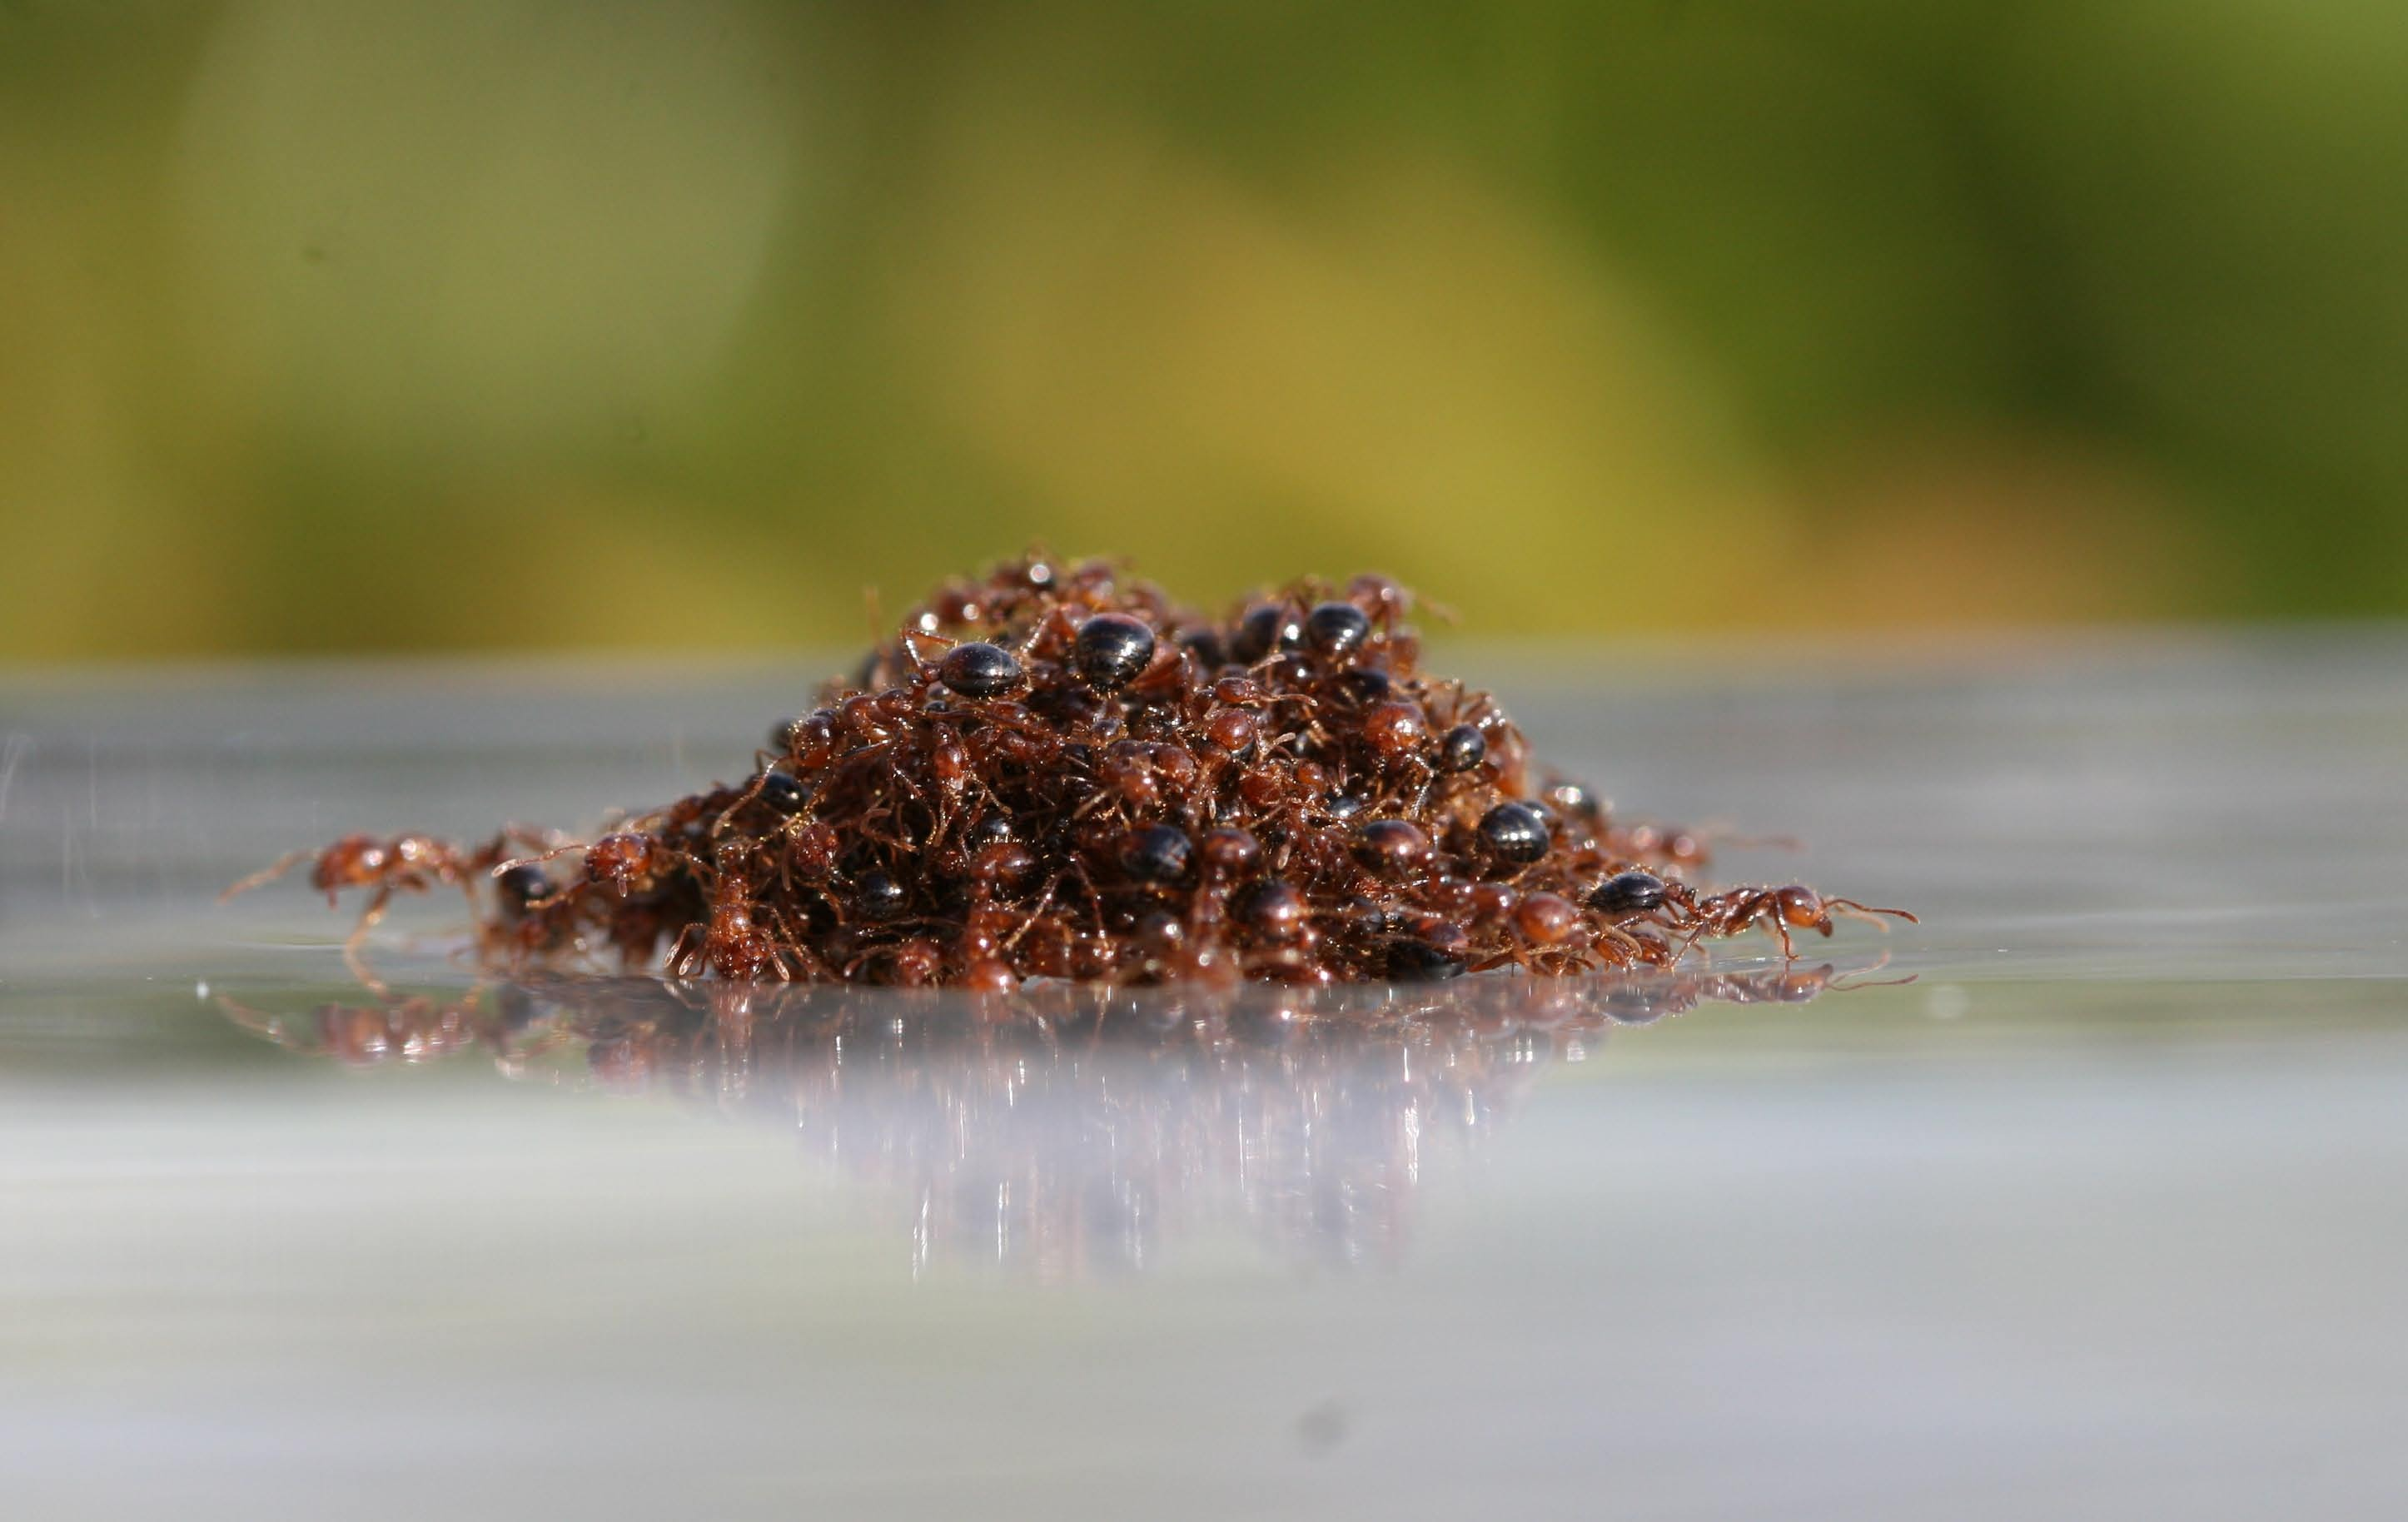
\includegraphics[width=4in]{figures/binary/ants}
    \caption{A raft of 500 fire ants, reproduced from
      \citet{mlot11}.\label{fig:ants}}
    \end{center}
\end{figure}
\end{acknowledgments}
